\section{Codereview-Tools}
\label{sec:Coderview}
\unsure{IDE Tools und  Static analysis tools erwähnen}
\unsure{Beschreibe die Arten von CRSs 1) post-commit 2) pre-commit 3) pull-requests}

\section{Codereview-Systeme, die Git unterstützen}
\label{sec:CRS-Git}

\subsection{Bitbucket}
\label{subsec:Bitbucket}
Bitbucket ist ein Git Code-Management. Bitbucket unterstützte nach seinem Entwurf als \ac{VCS} nur Mercurial. 
Erst in 3 Jahren später wurde um die Unterstützung von Git erweitert. Am 1. Juni 2020 wurde die Unterstützung von Mercurial vollständig eingestellt.
Die Review in Bitbucket erfolgt durch eine Pull-Anfrage.
	
\begin{figure}[h]
	\centering
	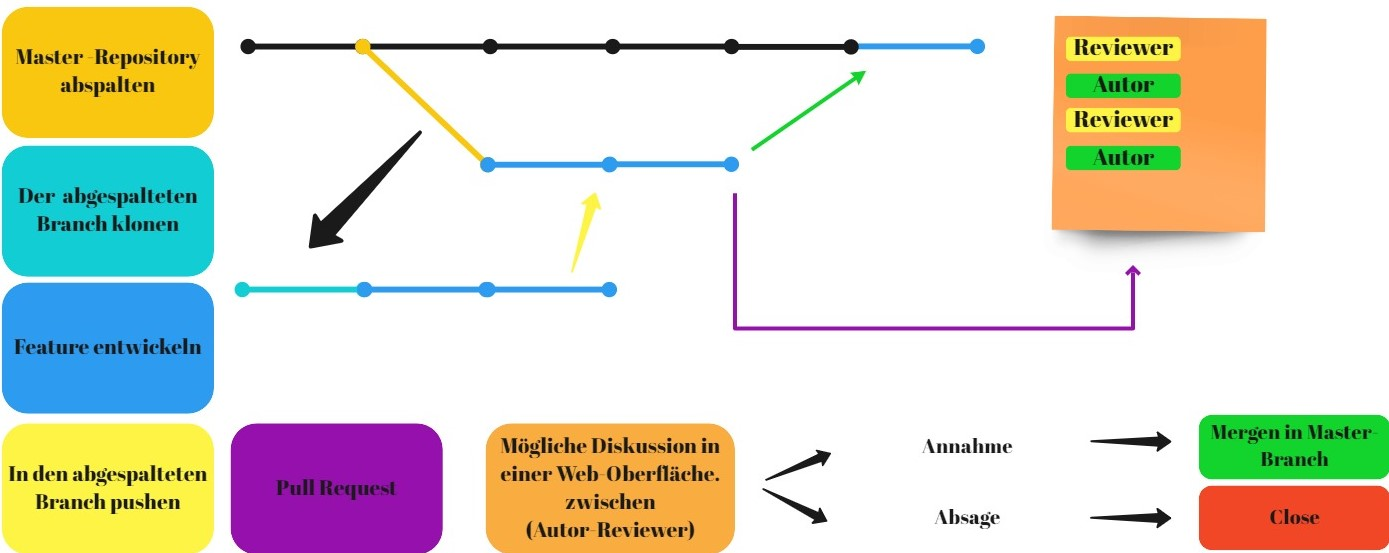
\includegraphics[width=1.0\textwidth]{Bitbucket_Forking-Workflorw}
	\caption[Bitbuckets Ablauf]{Bitbuckets Ablaufsmöglichkeit,\\ Quelle: eigene Darstellung}
	\label{fig:Bitbucket_Forking-workflow}
\end{figure}		  

\begin{description}
	\item{Vorteile:}
	\begin{enumerate}
		\item Unbegrenzte Anzahl von private Repositories.
		\item Hosting in Cloud oder auf eigenem Server.
		\item \ac{CI}/\ac{CD} sind in Bitbucket integriert.
		\item Erstellen von einer Merge-Checkliste mit zugeordneten Genehmigern.
		\item Für kleine Teams (Bis 5 Personen) bestehen keine Kosten.
		\item Nettes Design.
	\end{enumerate}
	
	\item{Nachteile:}
	\begin{enumerate}
		\item Um zu hosten in Bitbucketsever steht für mehr als 5 Personen einen monatlichen Beitrag.\\ Und für Self-hosten (In eigenen Server) besteht eine einmalige Zahlung.\\
		Der Preis für beide Varianten variiert je nach Personenanzahl.
	\end{enumerate}
\end{description}

\subsection{Crucible}
\label{subsec:Crucible}
Art der Review: \textit{pre- and post-commit}. Crucible ist ein Atlassians Produkt, das eine Unkomplizierte, formelle Codereview anbietet.

\begin{description}
	\item{Vorteile:}
	\begin{enumerate}
		\item Review des Inhalts ist flexibel.
		\item Diskussionsrunden um in Bestimmten Quelltextzeilen Dateien oder einen gesamten Änderungssatz zu Kommentieren.
		\item Nachverfolgen, Maßnahmen ergreifen in Bezug auf das, was der Autor wichtig findet.
		\item Ansicht vom Reviewstatus und wer möglicherweise Überprüfungen aufhält.
		\item Berichte über Stellen im Quelltext, die noch nicht überprüft wurden.
		\item unterstützt nicht nur Git sonder SVN auch.
	\end{enumerate}
	
	\item{Nachteile:}
	\begin{enumerate}
		\item Die Review muss manuell in Git eingefügt werden(Mergen ist nicht möglich).
		\item Schwer zu erzwingen (Der Autor muss nicht eine Review durchführen).
	\end{enumerate}
\end{description}
